\chapter{Основные положения обучения с подкреплением}

% не рекомендуется использовать отдельную section <<введение>> после лета 2020 года
%\section{Введение. Сложносоставное название первого параграфа первой главы для~демонстрации переноса слов в содержании} \label{ch1:intro}

Цель главы -- дать общее представление о терминах и алгоритмах обучения с подкреплением. В параграфе \ref{ch1:sec1} приводится актуальность изучения новой области инженерами в области автоматизации. В параграфе \ref{ch1:sec2} приведены основные положения обучения с подкреплением в терминологии свойственной для специалистов в области искусственного интеллекта, именно на базе введенной в данном параграфе терминологии формулируются методы и алгоритмы обучения с подкреплением в параграфе \ref{ch1:sec6}.
%\textbf{1.1 Название параграфа} \label{ch1:sec1}
%\addcontentsline{toc}{section}{\hspace{42pt} 1.1 Название параграфа}
\section{Актуальность обучения с подкреплением}
\label{ch1:sec1}

Обучение с подкреплением (англ. Reinforcement learning, RL) -- это широкая область, объединяющая исследователей из самых разных областей: искусственный интеллект (ИИ), управление, робототехника, исследования операций, экономика, нейробиология. По данной теме было опубликовано множество книг и обзорных статей представляющих самые разные области: ИИ, где классический учебник -- это учебник Саттона и Барто (1998) \cite{sutton1998introduction} со вторым изданием \cite{sutton2018reinforcement}, но также и другие \cite{littman1996reinforcement,van2012reinforcement}; теория управления \cite{lewis2012reinforcement}; оптимальное управление \cite{bertsekas1996neuro, powell2007approximate}; робототехника \cite{deisenroth2013survey}; Некоторые исследования сосредоточены на конкретных задачах RL: как методы градиента стратегии, аппроксимация функций, байесовские формулировки RL, иерархический RL, многоагентные подходы, глубокий RL, безопасный RL и так далее.

Необходимо упомянуть о том, что количество приложений методов RL для разработки систем управления техническими объектами мало в сравнении с количеством и масштабам приложений в области разработки рекомендательных систем, игр, обработки информации и исследований операций.

С одной стороны сложность применения к техническим системам затруднена в силу сложности обеспечения безопасности. В отличие от симуляции, в физическом мире действия имеют реальные последствия. В результате любой алгоритм, развернутый в реальных системах, должен отвечать нормам безопасности и качества. Безопасность в известных средах давно рассматривается и формализуется сообществами контроля и формальных методов, где можно синтезировать стратегии контроля, соответствующие заданной спецификации. Все методы определения устойчивости в области управления направлены на работу с моделями объектов. Тогда как при применении RL нет необходимости в математическом моделировании объекта.  основаны на известной модели системы.

Другая сложность RL для специалистов в области управления -- особенность терминологии и акцента на данные, которые привычны специалистам в области ИИ. Несмотря на эти и другие сложности, наблюдается рост исследований методов RL со стороны инженеров систем управления. Это подтверждается увеличением количества докладов и статьей, опубликованных в профильных журналах по автоматическому управлению (\firef{fig:pop-ch1}). Международная федерация по автоматическому управлению на конгрессе в 2020 году (IFAC-V 2020) вынесла на пленарное заседание доклад <<Reinforcement Learning for Process Control and Beyond>> (автор Jay H. Lee), что говорит о важности и влиятельности области обучения с подкреплением.
%
\begin{figure}[htb!] 
	\center
	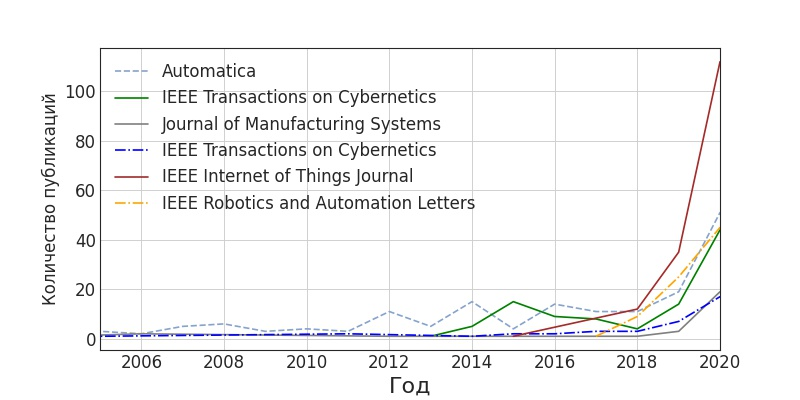
\includegraphics [scale=0.5] {my_folder/figure/schema/1.jpg}
	\caption{Тенденции количества публикаций на тему RL в специализированных журналах по управлению в технических системах} 
	\label{fig:pop-ch1}  
\end{figure}

Учитывая существующий запрос  на разработку интеллектуальных систем управление, что связано с возрастающей сложностью объектов управления, можно предполагать, что регуляторы с применением обучения с подкреплением станут неотъемлемой частью любого автоматизированного технологического процесса.
%


\section{Терминология обучения с подкреплением} \label{ch1:sec2} % ~ нужен, чтобы избавиться от висячего предлога (союза) в конце строки

Обучение с подкреплением -- это класс методов машинного обучения, которые основанны на взаимодействии алгоритма со средой и изменения стратегии действия или политики управления на основе стимулов, полученных в ответ на действия алгоритма, с целью получения желаемого результата. Цель применения методов RL — определить последовательность входных сигналов, которая обеспечивает желаемую работу динамической системы, начиная с минимальных знания о работе системы.

Агент -- интеллектуальная сущность (система/робота/алгоритм) принимающая решения, взаимодействует с объектом, который называется окружением или средой (англ., environment).  На каждом шаге последовательности $t = 0, 1, 2, ..$ агент и среда взаимодействуют. Среда или окружение задается, состоянием $S_t \in S$, где $S$ -- множество всех возможных состояний. Агенту в каждый момент времени в общем случае доступно только некоторое наблюдение (англ., observation) текущего состояния среды. На основании наблюдений состояния агент выбирает действия $A_t \in A(S_t)$, $A(S_t)$ -- множество действий, которые доступны агенту в состоянии $S_t$. Процедура выбора действий агентом называются стратегией или политикой (англ., policy) и обозначается как $\pi_t$, описывая вероятность выбора действия $A_t = a$ в состоянии $S_t = S$. По результатам применения действия $A(S_t)$ в среде, на вход агента поступает численная награда $R_{t+1} \in R$ (англ. reward) и новое состояние среды $A(S_{t+1})$. Методы RL определяют способ выбора стратегии агентом в результате полученного опыта.

Необходимо уточнить, что понимается под термином окружающая среда -- это все то, что не является агентом. На вход среды поступает действие агента, на выходе -- вознаграждение агента и состояние среды. 

\textit{Марковские процессы}. Одна из структур для RL основана на марковских процессах принятия решений (МППР). Задача RL удовлетворяет условию Марковости -- процесс зависит только от текущего состояния и не зависит от всей предыдущей истории. МППР позволяет формализовать основные элементы RL, такие как функции ценности, награды, а далее основные алгоритмы RL. Многие задачи принятия решений могут быть сформулированы как МППР, включая системы управления с обратной связью.
МППР представляет собой четверку $(S, A, P, r)$, где:

$S$ – конечное пространство состояний;

$A$ – конечное пространство действий;

$P$ – функция переходов, определяющая вероятность перейти в состояние $s'$ из состояния $s$ посредством действия $a$;

$r$  – функция награды.
При условии любого состояния $s$ и действия $a$, вероятность каждого возможного следующего состояния равна:
\begin{equation*}
p_{ij}(a, t) = P\{s_{t+1}=j|s_t=i, a_t=a\}
\end{equation*}
На рис. \ref{fig:intro} представлена общая структурная схема RL в терминах МППР.
\begin{figure}[ht!] 
	\center
	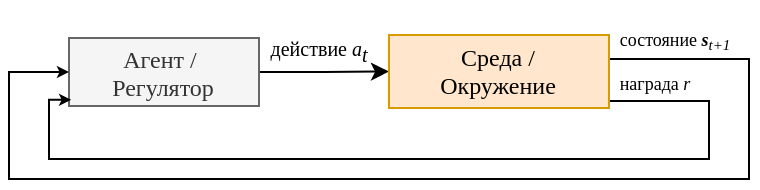
\includegraphics [scale=0.5] {my_folder/figure/schema/intro.png}
	\caption{Общая структура обучения с подкреплением} 
	\label{fig:intro}  
\end{figure}

В задаче обучения с подкреплением, цель агента формализуется в сигнале награды, которую получает агент от среды на каждом временном шаге. Использование сигнала награды для формализации цели -- одна из отличительных характеристик задачи обучения с подкреплением. Алгоритмы RL оптимизируют ту награду, которая была предоставлена ему на входе, при этом принимая истинной  <<гипотезы награды>>, которая утверждает, что любую интеллектуальную задачу можно определить (задать) при помощи функции награды. Но, как несложно догадаться, на практике дизайн функции награды оказывается сложной задачей и качество работы алгоритмы, напрямую зависит от способности формализовать цель управления.

Введено обозначение последовательности наград после временного шага $t$ -- $r_t, r_{t+1} ...$. Тогда в рамках задачи обучения с подкреплением, необходимо максимизировать ожидаемую награду $R_t$, которая равна сумме всех последующих наград. Тогда цель обучения с подкреплением, может быть сформулирована как максимизация ожидаемой награды $R_t$, которая задана как сумма всех последующих наград:
%
\begin{equation*}
R_t = r_t + r_{t+1} +  r_{t+2} + ... 
\end{equation*}
%
Такое выражение удовлетворительно для задач с конечным временным шагом,
В системах с конечным количеством шагов взаимодействия, вводится понятие разбиения взаимодействие агента и окружения на последовательности -- эпизоды. Каждый эпизод заканчивается особым терминальным состоянием, после которого осуществляется переход к заданному начальному состоянию или к выбору начального состояния из распределения начальных состояний. Среда называется эпизодичной, если для любой стратегии процесс взаимодействия гарантированно завершается не более чем за некоторое конечное число шагов.

Для ряда задач управления характерно продолжительное действие -- взаимодействие агента и окружения не разбивается на эпизоды. В этом случае ожидаемая награда, которую необходимо максимизировать, может достигать бесконечности. Для решения таких задач вводится коэффициент обесценивания (дисконтирования), тогда награда формируется следующим образом:
\begin{equation*}
R_t = r_t + \gamma r_{t+1} + \gamma^2 r_{t+2} + ... + \gamma ^{k-1} r_{t+k-1}
\end{equation*}
где $\gamma \in (0, 1]$ -- коэффициент дисконтирования.

Предполагается, что на каждом шаге с вероятностью $1-\gamma$ взаимодействие обрывается, и итоговым результатом агента станет та награда, которую он успел собрать до прерывания.Это обеспечивает приоритет получению награды в ближайшее время перед получением той же награды через некоторое время. Математически смысл дисконтирования, во-первых, в том, что данный коэффициент позволяет гарантировать ограниченность оптимизируемого функционала, а во-вторых, выполнение условий некоторых теоретических результатов, которые явно требуют $\gamma < 1$.

Учитывая терминологию приведенную выше, задача RL для заданного МППР может быть сформулирована как поиск стратегии $\pi^*$, максимизирующей среднюю дискредитированную суммарную награду. 
\begin{equation}
\label{eq:fun-ch1}
J(\pi) = E_{\pi}\sum_{t=0}^{\infty}\gamma^{t}r(s_t, \pi(s_t)) \rightarrow \max_{\pi}
\end{equation}


В основе многих алгоритмов RL лежит понятие функции ценности и функции ценности действия. Это в некотором роде <<обобщение>> функционала \ref{eq:fun-ch1}, варьируя начальное состояние. \textit{Функция ценности} (англ. Value Function) или оценочная функция состояния $V^{\pi}(s)$ показывает сколько набирает в среднем агент из состояния $s_t$ при стратегии $\pi$. Функция ценности определяется для отдельных стратеги $\pi$ и равна сумме наград:
\begin{equation}
\label{eq:val-ch1}
V^{\pi}(s) = E_{\pi}\{R_t | s_t = s\} = E_{\pi} \left[\sum_{t=0}^{\infty}\gamma^{t}r(s_t, \pi(s_t))\Bigg|s_t = s \right]
\end{equation}
где $E_{\pi}$ -- ожидаемое значение награды $R_t$ при действии агента в соответствии со стратегией $\pi$ на каждом $t$.

\textit{Функция ценности действия} $Q^{\pi}(s, a)$ (англ. Value Action) для стратегии $\pi$ характеризует сколько набирает в среднем агент из состояния $s_t$ после выполнения действия $a$. 
\begin{equation*}
Q^{\pi}(s, a) = E_{\pi}\{R_t | s_t = s, a_t = a\} = E_{\pi}\left[\sum_{t=0}^{\infty}\gamma^{t}r(s_t, \pi(s_t))\Bigg|s_t = s, a_t = a\right]
\end{equation*}

Функцию ценности и функцию ценности действий также называют V-функцией и Q-функцией, соответственно.

Исходя из задания V-фунции \eqref{eq:val-ch1} задача RL формулируется как определение политики $\pi(s,a)$, которая максимизирует награду: 
\begin{equation*}
\pi^{*}(s,a) = \underset{\pi}{\arg \max}  V_t^{\pi}(s) = \underset{\pi}{\arg \max }  E_{\pi} \left[\sum_{t=0}^{\infty}\gamma^{t}r(s_t, \pi(s_t))\Bigg|s_t = s \right]
\end{equation*}

Политика $\pi^{*}(s,a)$ называется оптимальной политикой, и соответствующее оптимальное значение V-функции задается как:
\begin{equation*}
V_t^{*}(s) = \underset{\pi}{\max }  V_t^{\pi}(s) = \underset{\pi}{\max }  E_{\pi} \left[\sum_{t=0}^{\infty}\gamma^{t}r(s_t, \pi(s_t))\Bigg|s_t = s \right]
\end{equation*}

Легко заметить, что для максимизации $V_t^{\pi}(s_0)$, где $s_0$ -- стартовое состояние, необходимо максимизировать $V_t^{\pi}(s)$. То есть задача имеет подзадачи эквивалентной структуры. Ряд методов RL основывается на рекурсивном свойстве V-функции. Тоже верно и для Q-функции. Это означает то, что для этих функций может быть записано уравнение Беллмана, которое выражает отношение между значениями функций в текущем состояний и значением в последующих состояний.
%
\section{Историческая справка}

Термин <<подкрепление>> (англ. reinforcement) унаследован из поведенческой психологии, а именно из работ физиолога И.П. Павлова. Здесь подкрепление обозначает награду или наказание за  результат, который зависит как от принятых решений так и от внешних, в общем случае, не контролируемых воздействий. Под обучением здесь понимается поиск способов достичь желаемого результата методом проб и ошибок, то есть попытки решить задачу и использовать накопленный опыта для усовершенствования своей стратегии выбора действий в будущем.

Специалисты в области обучения с подкреплением на раннем этапе истории выделяют два основных  направления развития. Одно направление связано с обучением методом проб и ошибок. И направление оптимального управления и решения задачи с применением динамического программирования.

Главной психологической идеей, которая используется в обучении с подкреплением, является метод проб и ошибок, предложенный ученым и философом Александром Бэном в 1855 году. Ученый объясняет возникновение произвольных движений -- вводит представление о спонтанной активности нервной системы. Если движение более одного раза совпадает с состоянием удовольствия, то некоторая <<сила>> устанавливает между ними связи. На базе идеи метода проб и ошибок начиная с 1930 годов было сделано ряд автоматов, демонстрирующий этот подход. Самая ранняя демонстрация — машина Томаса Росса 1933-ого года, которая могла пройти простейший лабиринт и запомнить последовательность переключателей. В 1952 году Клод Шеннон продемонстрировал лабиринт с роботом-мышью, который передвигался по лабиринту с помощью трех колес и магнита с обратной стороны лабиринта, он мог запомнить путь по лабиринту, исследуя его тем самым методом проб и ошибок. Появление таких электро-механических машин открыло путь к написанию компьютерных программ, способных к разным типам обучения, некоторые из которых были способны к обучению методом проб и ошибок.

Независимо развивался подход оптимального управления. Термин «оптимальное управление» появился в конце 1950-х годов и применялся для описания задачи проектирования устройств управления,при условии максимизации заданной характеристики поведения динамической системы во времени. Один из ключевых подходов к решению задачи оптимального управления был разработан в середине 1950-х годов Ричардом Беллманом и другими учеными путем обобщения теории Гамильтона–Якоби, созданной в XIX веке. Данный подход основан на решении функционального уравнения Беллмана, и носит название -- динамическое программирование (ДП) \cite{bellman1957dp}.  Другое ключевое понятие, как уже было сказано ранее, -- это МППР. В работе \cite{bellman1957markovian} описана дискретная стохастическая версия задачи оптимального управления, известная под названием «марковский процесс принятия решений» (МППР, англ.  MDP).  В работе Ховарда Роналда \cite{howard:dp}  предложен  метод  итерации  по стратегиям  для  МППР.  
Все это –  ключевые элементы, которые лежат в основе обучения с подкреплением. Известно, что ДП –  единственный применимый на практике способ решения общих стохастических задач оптимального управления. Большим ограничением ДП является «проклятье размерности» -- требования к вычислительной мощности растут экспоненциально с ростом числа переменных состояния.  Несмотря на ряд ограничений и недостатков, связанных с сложностями хранения больших объемов и большими вычислительными затратами на расчеты, ДП гораздо более эффективно и распространено, чем любой другой общий метод. 

Развитие оптимального управления и обучения с подкреплением происходило независимо, так как данные области ставят перед собой разные цели. 
Так же влияет тот факт, что динамическое программировании  представляется как  пакетный  метод  вычислений,  который  сильно  зависит от  наличия  точной  модели  системы  и  аналитических  решений  уравнения  Беллмана. К  тому же  простейшая  форма  динамического  программирования – вычисление,  происходящее  в  обратном  направлении  по  времени,  поэтому  трудно  понять, как  его  можно  применить в  процессе  обучения, который  по  необходимости протекает  в  прямом  направлении. 

Некоторые  из  первых  работ  по  динамическому  программированию, содержат в себе и идеи обучения например  \cite{bellman1959functional}.  В  работе  \cite{werbos1987} приводятся  явные  аргументы  в  пользу  более  тесной  связи  между  динамическим программированием  и  методами  обучения  и  доказывается,  что  динамическое программирование  имеет  прямое  отношение  к  пониманию работы  нейронов и  когнитивных  механизмов.  


Явная связь методов  динамического программирования  с  обучением для дискретных стохастических систем отражена в работе  Криса  Уоткинса  1989  года \cite{watkins1989learning},  в  которой  обучение с  подкреплением изложено  с  позиций  формализма  МППР. Методы оптимального управления и обучения с подкреплением активно  разрабатываются  многими  исследователями, в  особенности  Димитрием Бертсеркасом  и  Джоном  Цициклисом, которые  предложили  термин  «нейродинамическое  программирование»,  описывающий  комбинацию динамического  программирования  с  нейронными  сетями \cite{bertsekas1996neuro}. Еще  один  термин,  широко  употребляемый  в  настоящее  время, -–  «приближенное (адаптивное) динамическое  программирование».  



\section{Примеры применения обучения с подкреплением}
Первоначально методы RL применялись только к простым задачам, но применение глубоких нейронных сетей позволило применять RL для систем другого уровня сложности. Сейчас RL применяется в самых разных областях: робототехника, финансы, автономные транспортные средства, медицина и здравоохранения, оптимизация процессов и обнаружение неисправностей. Ниже рассмотрены основные области применения RL:
\begin{itemize}[]
	\item Промышленная робототехника -- активно развивающаяся область применения RL, поскольку является естественным внедрением этой парадигмы в практику \cite{kober2013reinforcement}.
	Например, использование глубокого обучения и обучения с подкреплением позволяет обучать роботов, способных захватывать различные объекты - даже те, которые не видны во время обучения. Или другой пример -- обучение работа повторять команды за человеком, выполняя перемещение объектов \cite{ml3}. Данные приложения могут быть использованы при сборке продуктов на сборочной линии. 
	
	
	\item Здравоохранение. RL в здравоохранении относится к методам динамического лечения (англ. Dynamic Treatment Regimes), так как алгоритмы RL позволяют находить решения для оптимального лечения пациентам в каждый момент времени. Например, вход алгоритма  -- набор клинических наблюдений и оценок пациента, выход - варианты лечения для каждого этапа.\cite{yu2019reinforcement}
	
	\item Обработка естественного языка. RL активно применяется при решении таких задач, как построение диалоговых систем \cite{li2016deep}, резюмированние и сокращение текстов \cite{paulus2017deep} машинный перевод и др.
	
	\item Проектирование архитектуры глубоких нейронных сетей. С одной стороны, применение RL для подбора архитектуры -- вычислительно затратное решение, но такой подход позволяет создавать лучшие архитектуры глубоких нейронных сетей.
	
	\item Автономные транспортные средства. Алгоритмы RL используются как для организации дорожного движения - автономные светофоры, так и для решения задач автономного вождения, например, оптимизация траектории движения, динамическое определение пути, смена полосы движения, парковка \cite{talpaert2019exploring}.
	
	\item Оптимизация производственных процессов.  RL применяется для прогнозирования технического обслуживания, диагностики оборудования режиме реального времени и управлять производственной деятельностью, а так же для оптимизации энергопотребления.\cite{waschneck2018optimization}
	Например, компания Royal Dutch Shell применяет RL в задачах по разведке и бурению. Алгоритмы RL, обученные на исторических данных бурения, а также дообученные на физических моделях, используются для управления газовыми буровыми установками при их движении по геологической среде.
\end{itemize}
%
%
\section{Классификация алгоритмов обучения с подкреплением}
В данном разделе приведена основополагающая классификация алгоритмов RL. На \firef{fig:classification-ch1} представлена лишь одна из возможных таксономий алгоритмов RL. Одна из наиболее важных классификаций основана на наличии доступа или возможность исследования агентом модели среды.\\
\begin{figure}[!h]
	\centering
	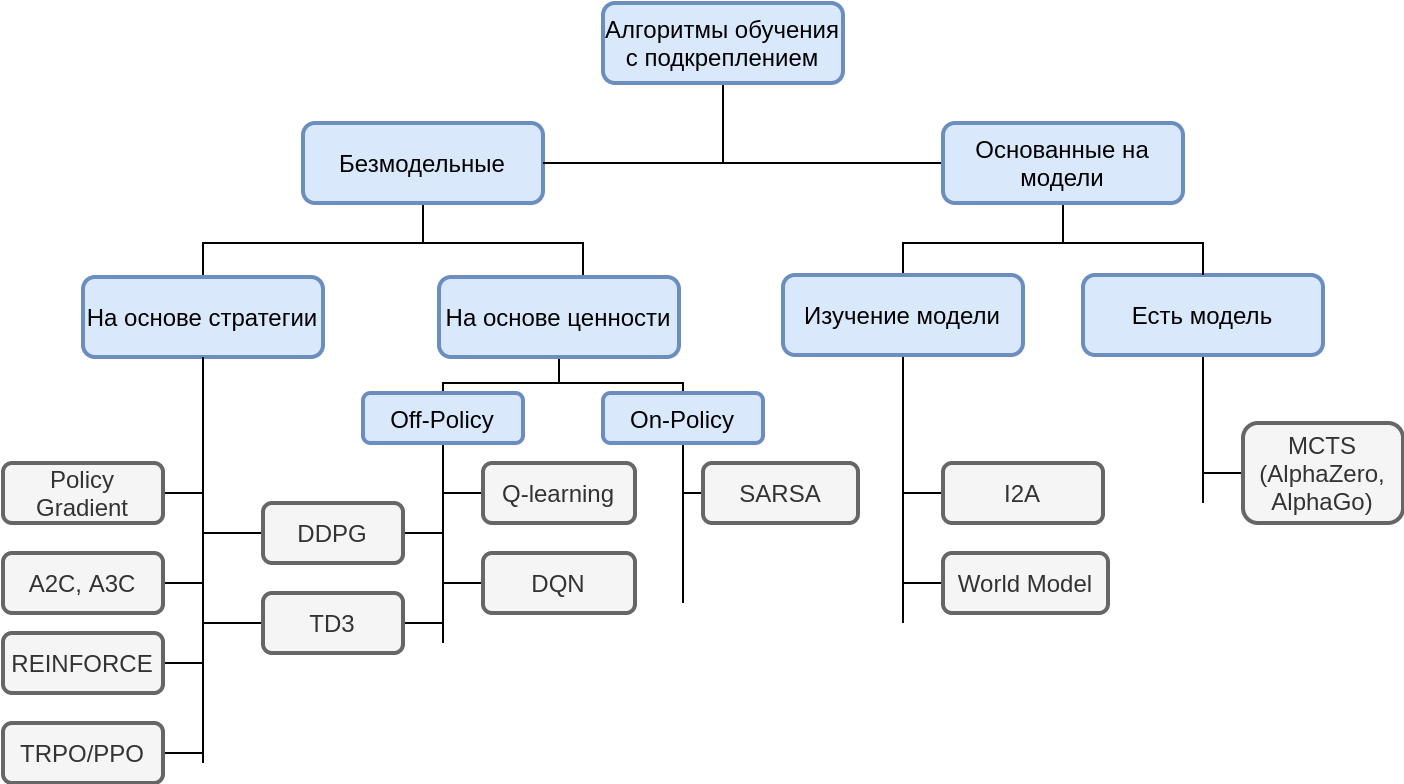
\includegraphics[width=0.7\linewidth]{my_folder/figure/schema/classification_RL.png}
	\caption{Классификация алгоритмов Rl}
	\label{fig:classification-ch1}
\end{figure}

Алгоритмы модельно-ориентированного обучения (англ. model-based RL) на первом этапе решают задачу идентификации системы либо используют уже составленную модель для решения задач управления. Безмодельное обучение (англ. model-free RL) направленно на прямой поиск управления на основе наблюдений и действий. Другими словами, безмодельные методы направлены на решение задач управления путем исследования системы и улучшения стратегий на основе прошлых вознаграждений и состояний. Модельные алгоритмы RL имеют такой же недостаток, как и классические подходы в управлении -- сложность получения достоверной модели среды (объекта).

Безмодельные методы в свою очередь делятся на два подхода: оптимизация политики  и на основе функции ценности. Алгоритмы градиента стратегии (англ. Policy-based) , использую оценки градиента функционала по параметрам политики, что означает, что каждое обновление использует данные, полученные на последней политики. Алгоритмы на основе ценности (англ. value-based) позволяют получать стратегию неявно через теорию оценочных функций. В наиболее часто встречающейся постановке для аппроксимации функции применяются глубокие нейронные сети и другие современные подходы, которые позволяют справиться с высокой дисперсией и общей неустойчивостью. 
Стоит отметить, что алгоритмы градиента стратегии применимы для сред с непрерывной областью действий, тогда как алгоритмы функций ценности применяются для дискретных систем. Поскольку такие алгоритмы используют целевую функцию основанную на уравнении Беллмана. Модельные и безмодельные алгоритмы не лишены недостатков, поэтому ведется активное развитие гибридных безмодельных алгоритмов RL.

Наколенные данные от эксперта, то есть записи взаимодействия со средой некоторой стратегии, не обязательно оптимальной, могут упростить задачу поиска условного оптимального решения ряда алгоритмов RL. Исходя из способности алгоритма использовать опыт взаимодействия со средой произвольной стратегии, выделяют on-policy и off-policy алгоритмы. Алгоритм off-policy способен использовать для обучения опыт взаимодействия произвольной стратегии. То есть появляется возможность проводить очередной шаг обучения на произвольных траекториях, сгенерированных произвольными стратегиями. Для алгоритма on-policy на очередной итерации требуется опыт взаимодействия конкретной, предоставляемой самим алгоритмом, стратегии. В то же время, накопленные данные от эксперта могут быть использованы для инициализации on-policy алгоритмов. Важно, что off-policy алгоритмы способны на данных произвольного эксперта условно сойтись к оптимуму при достаточном объёме и разнообразии экспертной информации, не требуя дополнительного взаимодействия со средой.



\section{Методы и алгоритмы обучения с подкреплением}
\label{ch1:sec6}
\textit{Динамическое программирование}. Динамическое программирование (ДП) -- один из фундаментальных модельных методов в RL, который основан на уравнении Беллмана. Базовыми алгоритмами ДП являются итерирование стратегий (англ., Policy iteration, PI)  и итерирование ценности (англ., Value iteration, VI). Алгоритм PI во время одной итерации вычисляет функцию награды для текущей стратегии, потом улучшает эту стратегию, то есть оценивание и улучшение стратегии выполняется циклически, тогда как в алгоритме VI -- оценивание и улучшение стратегии выполняется за одно обновление.
В литературе по RL процесс вычисления функции ценности состояния $V^{\pi}$ для произвольной стратегии $\pi$ называют оценкой стратегии (англ. Policy Evaluation) или задачей прогнозирования. Вычисление функции ценности необходимы для того, чтобы далее найти улучшенную стратегию управления. Процесс формирования новой, улучшающей исходную, стратегии называется улучшением стратегии (англ., Policy Improvement). Так, вычисленное значение функции ценности позволяет улучшить стратегию, в частности, жадной стратегией:
\begin{equation*}
\pi' = argmax_a Q_{\pi}(s, a) = argmax_a \sum_{s',r}p(s'|s,a)[r + \gamma V_pi(s')]
\end{equation*}

Алгоритм итерация по стратегиям представлен на \firef{fig:PI-ch1}. Алгоритм итерация по ценности представлен на  \firef{alg:VI}.
\begin{figure}[ht!]
	\begin{tcolorbox}
		\textbf{1. Инициализация} $V(s) \in \mathcal{R}$ и $\pi(s) \in \mathcal{A}(s)$ для всех $s \in \mathcal{S}$ \\
		\textbf{2. Оценка стратегии}
		Пока {$\Delta < \theta$}
		
		{$v:=V_k(s)$}
		
		{$V_{k+1}(s):=\sum_{s',r}p(s'|s,\pi(a))[r + \gamma V_k(s')]$}
		
		$\Delta := \max(\Delta, |v - V_{k+1}(s)|)$\\
		Конец цикла\\
		{\textbf{3. Улучшение стратегии}}\\
		{Стратегия устойчива:=истинно}\\
		Цикл {по $s\in\mathcal{S}$}
		
		{$b:=\pi(s)$}
		
		{$\pi(s) = argmax_a Q_{\pi}(s, a) = argmax_a \sum_{s'r}p(s'|s,a)[r + \gamma V_{k+1}(s)$]}
		
		Если {$b\neq \pi(s)$} тогда
		
		Стратегия устойчива:=ложно\\
		Конец цикла\\
		Если Стратегия устойчива тогда
		
		выход\\
		иначе переход к шагу 2
		
	\end{tcolorbox}
	\caption{Алгоритм итерирование стратегии}
	\label{fig:PI-ch1}
\end{figure}



\begin{figure}[ht!]
\begin{tcolorbox}
 \textbf{1. Инициализация} $V_0(s)$  произвольно для всех $s \in \mathcal{S}$\\ 
{\textbf{2. Оценка стратегии}}\\
Пока {$\Delta < \theta$}

{$v:=V_k(s)$}

{$V_{k+1}(s):=\sum_{s',r}p(s'|s,\pi(a))[r + \gamma V_k(s')]$}

$\Delta := \max(\Delta, |v - V_{k+1}(s)|)$\\
Конец цикла\\
{\textbf{3. Улучшение стратегии}}\\
{$\pi(s) = argmax_a \sum_{s'r}p(s'|s,a)[r + \gamma V_{k+1}(s)]$}\\

\end{tcolorbox}
	\caption{Алгоритм итерирование ценности}
	\label{alg:VI}
\end{figure}
%

%Асинхронное динамическое программирование
Недостатком методов ДП является то, что они требуют вычислений в каждом состоянии. В случае, если множество состояний велико, это может потребовать больших вычислительных ресурсов.
Асинхронные алгоритмы ДП обновляют оценки значений только подмножества состояний, а не всего набора на каждой итерации оценки политики. Такие алгоритмы обновляют значения состояний в любом порядке, используя значения других доступных состояний.
Как было сказано ранее, схема алгоритма PI состоит из двух чередующихся взаимодействующих шагов: оценка и улучшение стратегии. Шаг оценки стратегии устанавливает связь функции ценности с текущей стратегией. Шаг улучшения стратегии делает стратегию жадной к текущей функции ценности. В алгоритме VI между двумя улучшениями стратегии только одна итерация оценивания стратегии. В асинхронных методах ДП процесс оценивания и улучшение стратегии разбивается на более крупные чередующиеся итерации.

Одни из главных недостатков ДП -- экспоненциальное возрастание сложности вычислений с увеличением числа состояний (<<Проклятье размерности>>) и необходимость модели объекта. Несмотря на это, идеи оценки стратегии и итерирования по стратегии лежат в основе почти всех алгоритмов ОП.

В отличии от ДП методы Монте-Карло (МК) не предполагают полного знания о модели. Такие методы предполагают наличие данных -- набор состояний, действий и наград, полученных при взаимодействии с средой. Для применения методов МК требуется, чтобы задача была эпизодическая, так как методы МК инкрементны на уровне эпизодов, а не на уровне шагов. В отличии от ДП оценка для каждого состояния в методах МК -- независимы.
Подробно не будет останавливаться на методах МК и ДП.
%
%

\textit{Обучение на основе временных различий}.
Обучение на основе временных различий (англ., Temporal Difference, TD) или TD-обучение -- это метод обучения с подкреплением без использования моделей, где агент обучается на каждом отдельном действии, которое он предпринимает и при этом обновляет знания агента на каждом временном шаге (действии), а не в каждом эпизоде.TD-методы совмещают в себе идеи методов МК и ДП. Коррекция в простейшем TD-методе производится путем улучшения ценности на небольшую величину в направлении оптимального значения:
\begin{equation*}
\label{td_function}
V(s_t) = V(s_t) + \alpha[r + \gamma V(s_{t+1}) - V(s_t)]
\end{equation*}
где $\alpha$ -- параметр, который определяет степень изменения ценности состояния при каждом обновлении. Если $a = 0$, то ценность состояния не изменяется. Если же $a = 1,$ то ценность состояния будет равна $r + \gamma V(s_{t+1})$ -- старая ценность затирается. К алгоритмам TD-методов относятся: Q-learning, SARSA, R-learning, методы исполнитель-критик

На рис.\ref{fig:q_learn-ch1} -- \ref{fig:sarsa-ch1} представлены алгоритмы Q-learning, SARSA. Алгоритм Q-learning -- это табличный безмодельный off-policy алгоритм RL. Это метод основан на временных разностей для вычисления оптимальной Q-функции с $\varepsilon-$жадной стратегией исследования, то есть агент выбирает случайное действие с вероятностью $\epsilon$, но использует известное лучшее действие. Алгоритм наследует от TD-обучения характеристики одношагового обучения, такие как возможность обучаться на каждом шаге и способность обучаться на опыте, не имея модели окружающей среды.
Q-learning отличается от SARSA прежде всего тем, что это алгоритм с разделенной стратегией. Разделенная стратегия означает, что обновление производится независимо от того, какая стратегия использовалась для накопления опыта, то есть алгоритмы с разделенной стратегией
могут использовать прежний опыт для улучшения стратегии. Стратегия, которая применяется для улучшение стратегии -- целевая, а стратегия для взаимодействия с окружающей средой -- поведенческая.
Алгоритм состоит из следующих шагов: 1. Инициализация Q-таблицы с нулевыми значениями, то есть в начальный момент времени все стратегии равновероятны и равноценны. 2. Выбор действия с наибольшей ценностью. 3. Отправка на вход среды выбранного действие, на выходе получаем вознаграждение. 4. Обновление Q-таблицы с учетом полученного вознаграждения.
Гиперпараметрами алгоритма являются $\alpha \in (0,1] $ -- параметр экспоненциального сглаживания, $\varepsilon > 0 $ -- параметр исследования.

	\begin{figure}[ht!]
		\centering
		\begin{tcolorbox}
\textbf{Инициализация} $Q(s, a)$ произвольно для всех $s \in \mathcal{S}$, $\alpha \in \mathcal{A}$\\
\textbf{Цикл} {по эпизодам}

\textbf{Инициализация} $s$

Цикл {по шагам эпизодов $k$}

\textbf{Выбор} $a_k$: с вероятностью $\epsilon$ принимаем $a_k \sim Uniform(\mathcal{A})$

 иначе $a_k = argmax Q(s_k, a_k)$
			
\textbf{Выполнение} действие $a_k$

\textbf{Нахождение} $r_k, s_{k+1}$

\textbf{Обновление} 

$Q(s,a ) \leftarrow Q(s, a) + \alpha [r_k + \gamma \max_{a_{k+1}}Q(s_{k+1}, a_{k+1})-Q(s_k,a_k)]$

\textbf{Конец цикла}\\
\textbf{Конец цикла}
		\end{tcolorbox}
		\caption{Алгоритм Q-learning}
		\label{fig:q_learn-ch1}
\end{figure}
%
\begin{figure}[!ht]
		\centering
		\begin{tcolorbox}%ht
\textbf{Инициализация} $Q(s, a)$ произвольно для всех $s \in \mathcal{S}$, $\alpha \in \mathcal{A}$\\
\textbf{Цикл} {по эпизодам}

\textbf{Считывание} $s_0$, находим $a_k \sim Uniform(\mathcal{A})$

\textbf{Цикл} {по шагам эпизодов $k$}

\textbf{Нахождение} $r_k, s_{k+1}$

\textbf{Выбор} $a_{k+1}$: с вероятностью $\epsilon$ принимаем $a_{k+1} \sim Uniform(\mathcal{A})$

иначе $a_{k+1} = argmax Q(s_{k+1}, a_{k+1})$
			
\textbf{Выполненине} действия $a_k$
			
\textbf{Обновление} 
$Q(s,a ) \leftarrow Q(s, a) + \alpha [r_k + \gamma Q(s_{k+1}, a_{k+1})-Q(s_k,a_k)]$

\textbf{Конец цикла}\\
\textbf{Конец цикла}
		\end{tcolorbox}
		\caption{Алгоритм SARSA}
		\label{fig:sarsa-ch1}
	\end{figure}

Разница между этими двумя алгоритмами в том, что SARSA выбирает действие, соответствующее той же текущей политике, и обновляет его Q-значения, тогда как Q-обучение выбирает жадное действие, то есть действие, которое дает максимальное значение Q для состояния, то есть оно следует оптимальной политике.

\textit{Аппроксимация V-функции}.

Главным недостатком перечисленных выше методов является необходимость хранить в памяти большие объемы данных при увеличении сложности объекта, а так же сложность работы с непрерывным пространством действий. Необходимо ввести аппроксимацию V-функции (Q-функции), что позволит представить функцию в  ограниченной области определения, располагая памятью фиксированного объема.Применение аппроксимации функций позволяет заменить
пространство состояний набором признаков, порождаемых по исходным со-
стояниям

Основная идея аппроксимации функций – воспользоваться набором при-
знаков для оценки значений V-функции (Q-функции). Есть несколько способов отобразить признаки на значения функции, например линейная аппроксимация, решающие деревья, алгоритм ближайших соседей, искусственные нейронные сети. В  случайно линейной аппроксимации функция ценности состояний записывается в виде взвешенной суммы признаков. Как можно ожидать, нейронные сети используются чаще других подходов. В частности, используются глубокие	нейронные сети (ГНС). 




%\begin{table} [htbp]% Пример оформления таблицы
%	\centering\small
%	\caption{Представление данных для сквозного примера по ВКР \cite{Peskov2004}}%
%	\label{tab:ToyCompare}		
%		\begin{tabular}{|l|l|l|l|l|l|}
%			\hline
%			$G$&$m_1$&$m_2$&$m_3$&$m_4$&$K$\\
%			\hline
%			$g_1$&0&1&1&0&1\\ \hline
%			$g_2$&1&2&0&1&1\\ \hline
%			$g_3$&0&1&0&1&1\\ \hline
%			$g_4$&1&2&1&0&2\\ \hline
%			$g_5$&1&1&0&1&2\\ \hline
%			$g_6$&1&1&1&2&2\\ \hline		
%		\end{tabular}	
%	\normalsize% возвращаем шрифт к нормальному
%\end{table}


% \firef{} от figure reference
% \taref{} от table reference
% \eqref{} от equation reference


%\FloatBarrier % заставить рисунки и другие подвижные (float) элементы остановиться

%\section{Выводы} \label{ch1:conclusion}



Вывод по главе \thechapter. В ходе анализа и изучения области обучения с подкреплением, сделаны следующие выводы:
\begin{itemize}

	\item МППР -- нотация для представления задачи обучения с подкреплением;
	\item Функция ценности и функция ценности действия -- основополагающие термины для дальнейших исследований; 
	\item Динамическое программирование рассматривается как один из главных способов обучения агента;
	\item Область управления и область обучения с подкреплением связаны математической базой, а именно уравнение Беллмана;
	\item Применение методов обучения с подкреплением распространено в области рекомендательных систем и игр;
\end{itemize}


%% Вспомогательные команды - Additional commands
%
%\newpage % принудительное начало с новой страницы, использовать только в конце раздела
%\clearpage % осуществляется пакетом <<placeins>> в пределах секций
%\newpage\leavevmode\thispagestyle{empty}\newpage % 100 % начало новой страницы